\section{Opera��es Suportadas}

Segue-se a descri��o de direc��es suportadas pelas opera��es, como ilustrado
na figura \ref{fig:shots}.

\subsection{Altera��o da Geometria}

\begin{figure}[!ht]
	\centering
	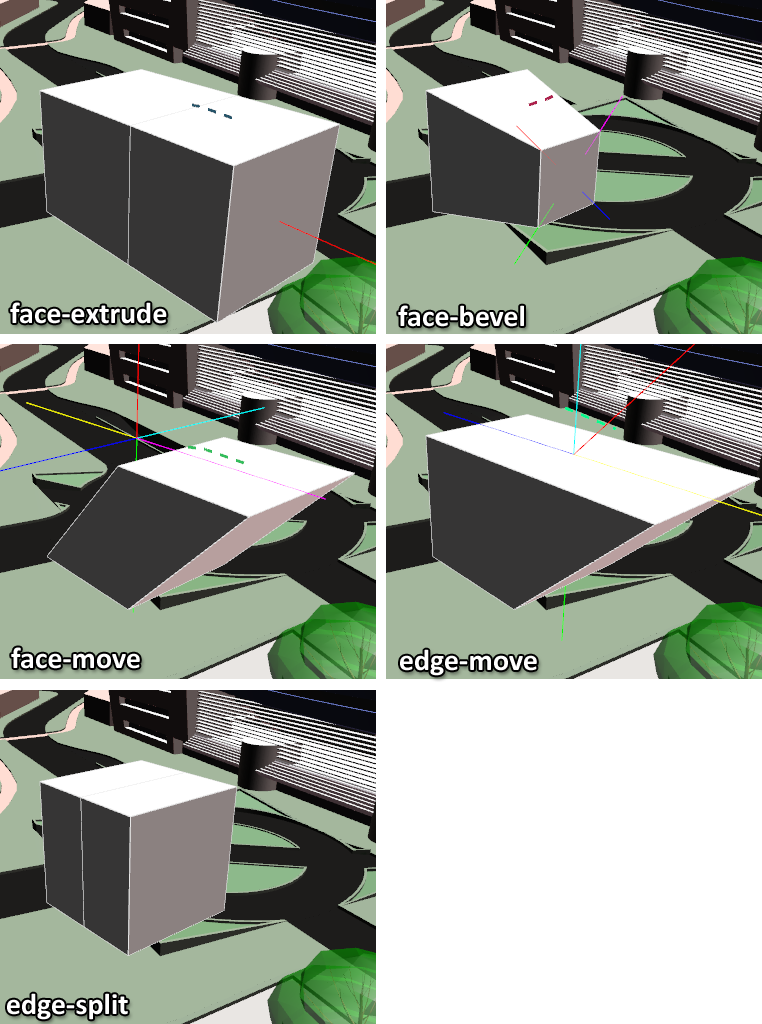
\includegraphics[width=0.9\linewidth]{shots2.png}
	\caption{opera��es no ImmiView}
	\label{fig:shots}
\end{figure}


\textbf{Extrus�o} --
a direc��o � definida pela compara��o com as normais exterior e interior da face origem.
O comprimento baseado no comprimento do tra�o.


\textbf{Bevel} --
a dimens�o do \textit{bevel} � dependente do comprimento do tra�o.


\textbf{Mover Face} --
suporta n�o s� as direc��es normais como tamb�m as co-lineares com as arestas fronteira da face.


\textbf{Mover Aresta} --
suporta para al�m das normais � aresta, as direc��es das faces vizinhas da mesma.


\textbf{Corte de Aresta} --
processa-se imediatamente, replicando o corte por arestas opostas at� terminar o \textit{loop} de face.

\subsection{Outras opera��es}

\textbf{Undo} --
um mecanismo de \textit{undo} foi implementado, baseado no padr�o de desenho
Memento \cite{despat}, capaz de armazenar a informa��o relevante sobre um objecto geom�trico,
tendo cada objecto associada uma pilha de estados de modo a poder regressar
a qualquer passo anterior de modela��o.

\textbf{Salvaguarda e Carregamento} --
uma forma geom�trica pode ser guardada para posterior carregamento num formato
XML definido. O mesmo segue o seguinte padr�o:
\begin{scriptsize}
	\begin{verbatim}
	<?xml version="1.0" encoding="utf-8"?>
	  <shape>
	    <vertices count="56">
	      <vertex x="-1" y="-0.627882" z="5.29942"/>
	      ...
	    </vertices>
	  <faces count="54">
	    <face v1="0" v2="1" v3="2" v4="3"/>
	    ...
	  </faces>
	  <colors count="54">
	    <color r="0.9" g="0.9" b="0.9"/>
	    ...
	  </colors>
	</shape>
	\end{verbatim}
\end{scriptsize}


